\documentclass[conference]{IEEEtran}
\IEEEoverridecommandlockouts
\usepackage[utf8]{inputenc}
\usepackage[T1]{fontenc}
\usepackage{amsmath,amssymb,amsfonts}
\usepackage{graphicx}
\usepackage{booktabs}
\usepackage{tabularx}
\usepackage{multirow}
\usepackage{microtype}
\usepackage[hidelinks]{hyperref}

\setlength{\textfloatsep}{5pt plus 1pt minus 1pt}
\setlength{\dbltextfloatsep}{5pt plus 1pt minus 1pt}
\setlength{\intextsep}{5pt plus 1pt minus 1pt}
\setlength{\abovecaptionskip}{2pt}
\setlength{\belowcaptionskip}{0pt}

\begin{document}

\title{Architectural Teardown and Parameter-Efficient Adaptation of DINOv2 for Spatial Generalization in Land Cover Classification}

\author{
\IEEEauthorblockN{Alfredo Jim\'enez}
\IEEEauthorblockA{\textit{Departamento de Ingenier\'ia} \\
\textit{Pontificia Universidad Cat\'olica del Per\'u}\\
Lima, Peru \\
alfredo.jf.2004@gmail.com}
\and
\IEEEauthorblockN{Jhonatan Davila}
\IEEEauthorblockA{\textit{Departamento de Ingenier\'ia} \\
\textit{Pontificia Universidad Cat\'olica del Per\'u}\\
Lima, Peru \\
jcdavilam@pucp.edu.pe}
\and
\IEEEauthorblockN{Italo Ramos}
\IEEEauthorblockA{\textit{Departamento de Ingenier\'ia} \\
\textit{Pontificia Universidad Cat\'olica del Per\'u}\\
Lima, Peru \\
italom.ramosd@pucp.edu.pe}
}

\maketitle

\begin{abstract}
Self-supervised vision foundation models such as DINOv2 learn rich representations from natural imagery, yet satellite scenes exhibit fundamentally distinct properties: nadir viewpoints, repetitive spatial textures, and subtle spectral boundaries. While linear probing preserves general features cheaply, it cannot adapt attention mechanisms to remote sensing textures; conversely, full fine-tuning is costly and risks regional overfitting. We present a three-phase study of DINOv2 ViT-S/14 on the 27,000-image EuroSAT Sentinel-2 benchmark. First, an instrumented teardown (Phase A) quantifies parameters, FLOPs, effective receptive fields, and token PCA, showing that semantic clustering concentrates in the deepest Transformer blocks. Second, injecting Low-Rank Adaptation (LoRA) strictly into query ($Q$) and value ($V$) projections of blocks 11--12 (Phase B) adds only 24,576 weights (0.11\% of the backbone) and raises internal macro-F1 from $95.66 \pm 0.16\%$ to $97.33 \pm 0.17\%$ across three seeds ($p < 10^{-4}$). Third, evaluating spatial out-of-distribution generalization across geographically disjoint European regions (Phase C) refutes regional overfitting: LoRA degrades significantly less than linear probing on unseen regions ($6.02\text{\,pp}$ vs.\ $7.15\text{\,pp}$), widening its advantage to $+2.27\text{\,pp}$ ($p < 10^{-6}$, exact McNemar test). Symmetric ablations confirm low intrinsic rank ($r=4$ suffices) and peak spatial transfer with four adapted blocks ($92.27\%$ out-of-region macro-F1), with zero inference latency overhead after weight merging.
\end{abstract}

\begin{IEEEkeywords}
DINOv2, Vision Transformer, LoRA, Remote Sensing, EuroSAT, Spatial Generalization, Architectural Teardown.
\end{IEEEkeywords}

\section{Introduction}
Self-supervised foundation models have transformed computer vision by producing general-purpose representations without manual labels. DINOv2~\cite{oquab2024dinov2}, a Vision Transformer (ViT)~\cite{dosovitskiy2021image} pre-trained on 142 million natural images (LVD-142M), achieves strong downstream accuracy under frozen linear probing. However, Sentinel-2 satellite tiles~\cite{drusch2012sentinel} differ markedly from web photographs: imagery is captured from overhead ($\sim$10\,m/px), lacks centered foreground objects, and separates land cover via distributed textures (e.g., crop parcels, rivers, highways, and urban blocks).

Assessing foundation feature transfer requires resolving two coupled issues: adapting representations parameter-efficiently without catastrophic forgetting, and verifying that improvements hold under geographic distribution shift rather than exploiting spatial autocorrelation in random splits~\cite{roberts2017cross}. Full fine-tuning updates all 22.06M parameters, risking regional overfitting. Low-Rank Adaptation (LoRA)~\cite{hu2022lora} constrains updates to low-rank subspaces and merges algebraically at zero inference overhead.

To determine whether LoRA improves land cover classification in unseen geographical regions compared to frozen DINOv2, we execute three structured phases:
\begin{itemize}
    \item \textbf{Phase A (Teardown):} Hardware and representational profiling of DINOv2 ViT-S/14 (parameters, FLOPs, latency, memory, effective receptive field, and token PCA).
    \item \textbf{Phase B (Intervention):} Controlled LoRA injection ($r=\alpha=8$) into $Q$ and $V$ of blocks 11--12 vs.\ linear probing under identical optimization budgets.
    \item \textbf{Phase C (Spatial Stress Test \& Ablations):} 20 idempotent runs across three seeds ($s \in \{0, 1, 42\}$) on geographically disjoint regions, paired exact McNemar testing, and ablations across rank, block depth, and projections.
\end{itemize}

\section{Dataset and Experimental Protocols}
\subsection{EuroSAT RGB Benchmark and Preprocessing}
We use the complete EuroSAT RGB dataset~\cite{helber2019eurosat}: 27,000 Sentinel-2 patches ($64\times64$\,px) across 10 land cover classes from 34 European countries (2,000--3,000 tiles per class; Fig.~\ref{fig:samples}). Tiles are resized to $224\times224$\,px via bicubic interpolation ($16\times16$ patches of 14\,px plus 1 \texttt{[CLS]} token, 257 tokens total) and normalized with ImageNet statistics. Center cropping is omitted since removing margins discards 23\% of scene texture. Following DINOv2 evaluation protocols~\cite{oquab2024dinov2}, classifier inputs concatenate the final LayerNorm \texttt{[CLS]} token and mean patch embedding ($d=768$), yielding a linear head of $7,690$ parameters.

\begin{figure}[t]
    \centering
    \includegraphics[width=0.86\linewidth]{../figures/00_muestras.png}
    \caption{Representative $64\times64$\,px Sentinel-2 RGB samples across the 10 EuroSAT classes.}
    \label{fig:samples}
\end{figure}

\subsection{Internal vs.\ Geographic Blocked Splits}
We evaluate under two complementary partitioning protocols:
\begin{enumerate}
    \item \textbf{Internal Stratified Split:} Random 70/15/15 split (18,900 train, 4,050 val, 4,050 test) preserving class proportions. This measures in-distribution adaptation where adjacent tiles can be spatially correlated.
    \item \textbf{Geographic Blocked Split:} Extracting exact EPSG:3035 UTM coordinates from georeferenced multispectral EuroSAT GeoTIFFs, we perform spatial $K$-means clustering ($K=12$ regions) with deterministic class-coverage constraints ($\ge 5\%$ per class per split). Held-out regions form \texttt{test\_fuera} (unseen geographical domains), while remaining clusters supply \texttt{train}, \texttt{val}, and in-domain \texttt{test\_dentro}.
\end{enumerate}

\section{Methodology}

\subsection{Phase A: Architectural Teardown}
We inspect \texttt{facebook/dinov2-small} (ViT-S/14 without registers~\cite{darcet2024vision}), whose Hugging Face implementation separates $Q$, $K$, and $V$ linear layers. It comprises 12 identical Transformer blocks ($d=384$, 6 heads, MLP hidden size 1,536), totaling 22,056,576 parameters (88.2\,MB in \texttt{fp32}; 1.78\,M/block: 67\% MLP, 33\% attention). Using eager attention with \texttt{torch.utils.flop\_counter} (1 MAC = 2 FLOPs), we profile compute across $112$\,px, $224$\,px, and $448$\,px inputs, compute gradient-based Effective Receptive Fields (ERF)~\cite{luo2016understanding}, and inspect top-3 PCA components of patch tokens across blocks 4, 8, and 12.

\begin{figure*}[t]
    \centering
    \includegraphics[width=0.78\linewidth]{../figures/B1_confusion_y_curvas.png}
    \caption{In-distribution evaluation (internal split, seed 42): confusion matrices for linear probing (left) and LoRA (center), alongside validation macro-F1 convergence over 8 epochs (right).}
    \label{fig:b1}
\end{figure*}

\subsection{Phase B: Controlled LoRA Intervention}
Because semantic information concentrates in deep layers, blocks 1--10 remain frozen while LoRA adapters are applied solely to $W_q$ and $W_v$ of blocks 11--12:
\begin{equation}
    h = W_0 x + \frac{\alpha}{r} B A x
\end{equation}
with frozen $W_0 \in \mathbb{R}^{384\times 384}$, Kaiming-uniform $A \in \mathbb{R}^{r\times 384}$, and zero-initialized $B \in \mathbb{R}^{384\times r}$ ($r=\alpha=8$, dropout $0.0$). This adds $24,576$ LoRA weights ($0.111\%$ of backbone; $32,266$ or $0.146\%$ including the head). Post-training, weights are merged ($W' = W_0 + \frac{\alpha}{r}BA$) for zero-overhead inference. Both linear probing (on cached frozen features) and LoRA share an identical budget: AdamW~\cite{loshchilov2019decoupled} ($\text{lr}=10^{-3}$, weight decay $10^{-4}$), batch 64, 8 epochs, mixed precision (\texttt{AMP}), and best validation macro-F1 selection.

\subsection{Phase C: Multi-Seed Stress Test and Ablations}
All primary experiments run across three seeds ($s \in \{0, 1, 42\}$) on both internal and geographic splits, verified via two-sided exact McNemar tests~\cite{mcnemar1947note}. Symmetric ablations ($s=42$) vary rank ($r \in \{4, 8, 16\}$), depth (4 blocks 8--11 vs.\ 2 blocks 10--11), and projections ($Q$-only vs.\ $Q+V$).

\section{Results and Discussion}

\subsection{Architectural Teardown (Phase A)}
Table~\ref{tab:teardown} profiles DINOv2 ViT-S/14 on an NVIDIA Tesla T4 GPU. At $224$\,px, forward inference takes 12.25\,GFLOPs (1.011\,GFLOPs/block), with quadratic attention representing 9.9\% of compute; scaling to $448$\,px raises cost $5.2\times$ to 63.36\,GFLOPs (30.6\% attention). Half-precision (\texttt{fp16}) inference at batch 128 achieves 1.17\,ms/img (853.7\,img/s) at 833\,MB peak VRAM.

\begin{table}[t]
\centering
\caption{DINOv2 ViT-S/14 Architectural Teardown (Tesla T4 GPU)}
\label{tab:teardown}
\footnotesize
\begin{tabularx}{\linewidth}{@{}lX@{}}
\toprule
\textbf{Metric} & \textbf{Measured Result \& Analytical Interpretation} \\
\midrule
Parameters & 22,056,576 (88.2\,MB fp32); 1.78\,M/block (67\% MLP, 33\% Attn). \\
FLOPs & 2.87\,G ($112$\,px), 12.25\,G ($224$\,px, 9.9\% Attn), 63.36\,G ($448$\,px). \\
Latency & fp32 b1: 8.89\,ms; fp16 b128: 1.17\,ms/img (853.7\,img/s). \\
Peak Memory & 187\,MB (b1, fp32) to 833\,MB (b128, fp32). \\
ERF (50\% Radius) & 69.4\,px (blk 1), 57.2\,px (blk 4), 67.3\,px (blk 8), 85.0\,px (blk 12). \\
\bottomrule
\end{tabularx}
\end{table}

\begin{figure}[t]
    \centering
    \includegraphics[width=0.86\linewidth]{../figures/A5_erf.png}
    \caption{Effective Receptive Field (ERF) across blocks 1, 4, 8, and 12. Global context emerges from block 1.}
    \label{fig:erf}
\end{figure}

As shown in Fig.~\ref{fig:erf}, self-attention yields a global ERF from block 1 ($50\%$ radius $=69.4\text{\,px}$). Patch-token PCA (Fig.~\ref{fig:pca}) reveals that block 4 encodes spatial grid coordinates, whereas block 12 separates semantic classes (e.g., roads vs.\ forest), justifying selective intervention in blocks 11--12. High-norm background tokens match register-free ViT artifacts~\cite{darcet2024vision}.

\begin{figure}[t]
    \centering
    \includegraphics[width=0.52\linewidth]{../figures/A4_pca_tokens.png}
    \caption{Top-3 PCA components of patch tokens across blocks 4, 8, and 12. Block 4 encodes position; block 12 groups semantic land cover.}
    \label{fig:pca}
\end{figure}

\subsection{In-Distribution Performance and Multi-Seed Robustness (Phase B)}
Across three seeds on the internal split (Table~\ref{tab:multiseed}), LoRA elevates macro-F1 from $95.66 \pm 0.16\%$ to $97.33 \pm 0.17\%$ ($+1.67\text{\,pp}$), cutting errors by $\sim$32\%. Paired exact McNemar tests confirm significance in every seed ($s=42$: $b=51, c=97, p=1.94\times10^{-4}$; $s=0$: $b=54, c=104, p=8.55\times10^{-5}$; $s=1$: $b=24, c=103, p=7.46\times10^{-13}$). Merged inference latency matches the frozen baseline ($4.41$ vs.\ $4.43\text{\,ms/img}$ at batch 32), while training takes $\sim$7$\times$ longer ($566\text{\,s}$ vs.\ $80\text{\,s}$). Fig.~\ref{fig:b1} shows that thin linear structures benefit most: Highway improves $+5.85\text{\,pp}$ and River $+3.71\text{\,pp}$ (River$\rightarrow$Highway errors fall from 21 to 2), while residual confusions occur among spectrally similar RGB vegetation classes.

\begin{table}[t]
\centering
\scriptsize
\setlength{\tabcolsep}{3.5pt}
\caption{Multi-Seed Macro-F1 ($s \in \{0, 1, 42\}$) Across Splits}
\label{tab:multiseed}
\begin{tabular}{@{}llccc@{}}
\toprule
\textbf{Split} & \textbf{Method} & \textbf{In-Domain} & \textbf{Out-Region} & \textbf{Drop ($\Delta$)} \\
\midrule
Internal & Linear probing & $95.66 \pm 0.16\%$ & --- & --- \\
Internal & LoRA (b11--12) & $\mathbf{97.33 \pm 0.17\%}$ & --- & --- \\
\midrule
Geo & Linear probing & $96.40 \pm 0.18\%$ & $89.25 \pm 0.72\%$ & $-7.15\text{\,pp}$ \\
Geo & LoRA (b11--12) & $\mathbf{97.54 \pm 0.17\%}$ & $\mathbf{91.51 \pm 0.38\%}$ & $\mathbf{-6.02\text{\,pp}}$ \\
\bottomrule
\end{tabular}
\end{table}

\subsection{Out-of-Distribution Geographic Generalization (Phase C)}
Table~\ref{tab:multiseed} and Fig.~\ref{fig:phasec}(a) present our core spatial generalization findings. Under geographic shift (\texttt{test\_dentro} $\rightarrow$ \texttt{test\_fuera}), frozen linear probing drops by $7.15 \pm 0.55\text{\,pp}$ (to $89.25\%$), whereas LoRA drops by only $6.02 \pm 0.55\text{\,pp}$ (to $91.51\%$). Rather than shrinking due to local overfitting---our pre-registered pessimistic hypothesis (H2, predicting $\le +0.5\text{\,pp}$)---LoRA \emph{doubles} its advantage in unseen regions from $+1.14\text{\,pp}$ to $\mathbf{+2.27\text{\,pp}}$, while nearly halving cross-seed variance ($\pm 0.38\%$ vs.\ $\pm 0.72\%$). Exact McNemar tests on \texttt{test\_fuera} yield $p=4.17\times10^{-10}$ ($s=42$), $p=2.86\times10^{-11}$ ($s=0$), and $p=6.07\times10^{-7}$ ($s=1$), formally rejecting H2 and demonstrating that LoRA acts as a spatial regularizer.

\begin{figure*}[t]
    \centering
    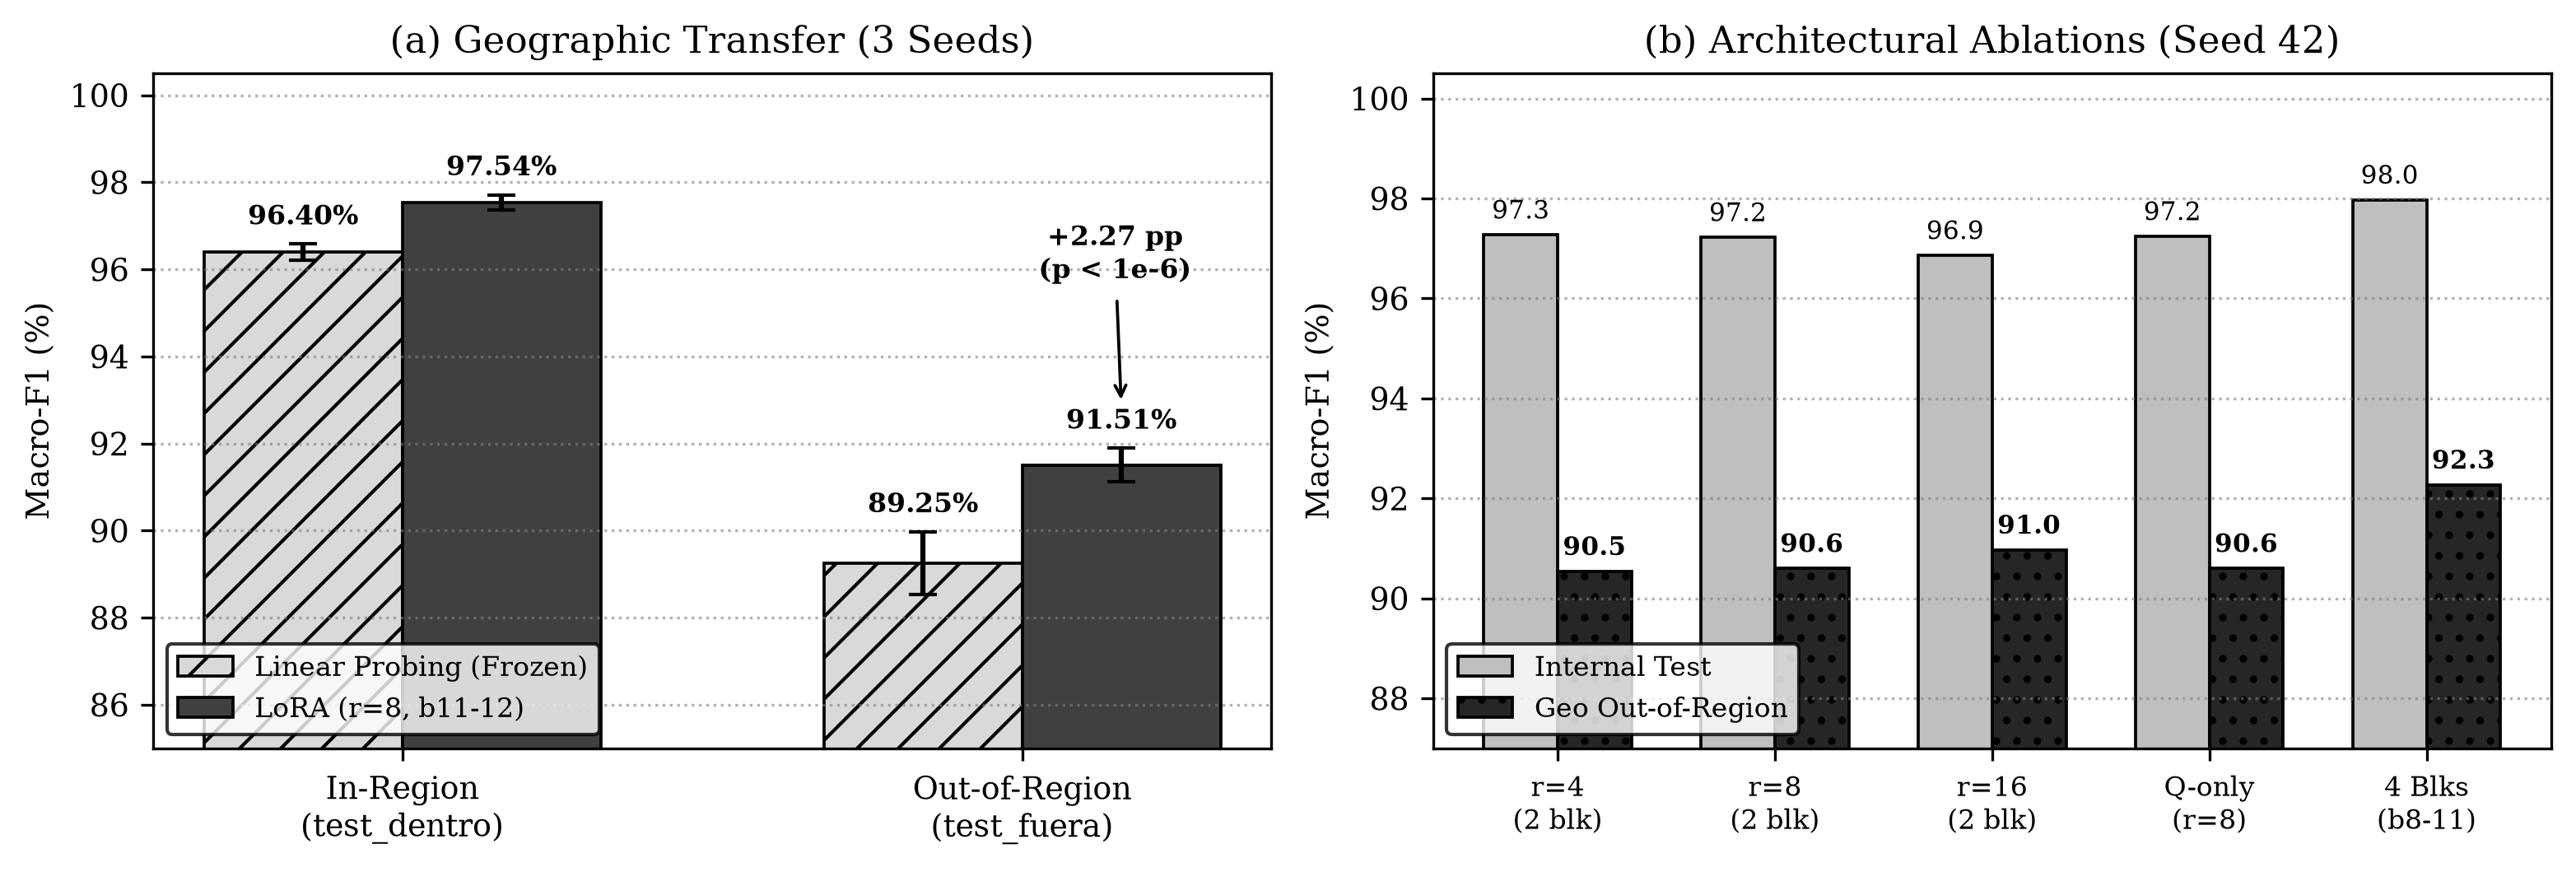
\includegraphics[width=0.76\linewidth]{../figures/C_fase_c_resultados.png}
    \caption{Phase C experimental summary: (a) mean $\pm$ std macro-F1 across 3 seeds comparing in-region vs.\ out-of-region geographic transfer; (b) symmetric architectural ablations across internal and out-of-region geographic splits (seed 42).}
    \label{fig:phasec}
\end{figure*}

\subsection{Architectural Ablations and Error Analysis}
Table~\ref{tab:ablations} and Fig.~\ref{fig:phasec}(b) summarize symmetric ablations ($s=42$):
\begin{itemize}
    \item \textbf{Rank Invariance:} $r=4$ achieves $97.27\%$ internal and $90.54\%$ out-of-region F1, matching $r=8$ ($97.22\%$, $90.60\%$) with half the adapter weights ($12,288$). $r=16$ yields no net gain ($96.86\%$ internal), confirming low intrinsic rank.
    \item \textbf{Depth Benefit:} Adapting four deep blocks (blocks 8--11) achieves peak performance across the study: $\mathbf{97.97\%}$ internal F1 ($98.05\%$ acc) and $\mathbf{92.27\%}$ out-of-region F1 ($94.88\%$ acc), maximizing resistance to spatial shift.
    \item \textbf{Projection Efficiency:} Tuning $W_q$ alone matches $Q+V$ ($97.24\%$ internal, $90.60\%$ geo) with $0.055\%$ backbone params.
\end{itemize}

\begin{table}[t]
\centering
\scriptsize
\setlength{\tabcolsep}{3.5pt}
\caption{Symmetric Architectural Ablations (Seed 42)}
\label{tab:ablations}
\begin{tabular}{@{}llrrr@{}}
\toprule
\textbf{Exp.} & \textbf{Configuration} & \textbf{LoRA Params} & \textbf{Int.\ F1} & \textbf{Geo-Out F1} \\
\midrule
A3 / A3g & $r=4$, b10--11, $Q+V$ & 12,288 (0.055\%) & 97.27\% & 90.54\% \\
Baseline & $r=8$, b10--11, $Q+V$ & 24,576 (0.111\%) & 97.22\% & 90.60\% \\
A3 / A3g & $r=16$, b10--11, $Q+V$ & 49,152 (0.222\%) & 96.86\% & 90.97\% \\
A5 / A5g & $r=8$, b8--11 (4 blks) & 49,152 (0.222\%) & \textbf{97.97\%} & \textbf{92.27\%} \\
A6 / A6g & $r=8$, b10--11, $Q$-only & 12,288 (0.055\%) & 97.24\% & 90.60\% \\
\bottomrule
\end{tabular}
\end{table}

Qualitative predictions (Fig.~\ref{fig:examples}) confirm that LoRA resolves fine linear structures (River vs.\ Highway), while residual errors stem from spectrally overlapping RGB vegetation textures.

\begin{figure}[t]
    \centering
    \includegraphics[width=0.88\linewidth]{../figures/C1_prediction_examples.png}
    \caption{Qualitative test predictions with softmax confidence: LoRA corrects linear River vs.\ Highway errors while fine vegetation overlaps remain challenging.}
    \label{fig:examples}
\end{figure}

\section{Conclusions and Future Work}
Adapting just 0.11\% of DINOv2 ViT-S/14 parameters via LoRA in the deepest attention blocks bridges the natural-to-satellite domain gap with zero runtime inference penalty after merging. Multi-seed geographic stress testing establishes that LoRA mitigates spatial domain decay ($-6.02\text{\,pp}$ vs.\ $-7.15\text{\,pp}$) and widens its out-of-region margin to $+2.27\text{\,pp}$ ($p < 10^{-6}$). Ablations show that rank $r=4$ and $Q$-only tuning suffice, while adapting four blocks maximizes spatial transfer ($92.27\%$ out-of-region F1). Future work will incorporate Sentinel-2 NIR/SWIR bands and evaluate register-equipped backbones.

\begin{thebibliography}{10}\setlength{\itemsep}{0pt}\setlength{\parskip}{0pt}
\bibitem{oquab2024dinov2} M. Oquab \emph{et al.}, ``DINOv2: Learning robust visual features without supervision,'' \emph{TMLR}, 2024.
\bibitem{dosovitskiy2021image} A. Dosovitskiy \emph{et al.}, ``An image is worth 16x16 words: Transformers for image recognition at scale,'' in \emph{Proc. ICLR}, 2021.
\bibitem{drusch2012sentinel} M. Drusch \emph{et al.}, ``Sentinel-2: ESA's optical high-resolution mission for GMES,'' \emph{Remote Sens. Environ.}, vol.~120, pp.~25--36, 2012.
\bibitem{hu2022lora} E. J. Hu \emph{et al.}, ``LoRA: Low-rank adaptation of large language models,'' in \emph{Proc. ICLR}, 2022.
\bibitem{helber2019eurosat} P. Helber \emph{et al.}, ``EuroSAT: A novel dataset and deep learning benchmark for land use and land cover classification,'' \emph{IEEE JSTARS}, vol.~12, no.~7, pp.~2217--2226, 2019.
\bibitem{darcet2024vision} T. Darcet \emph{et al.}, ``Vision transformers need registers,'' in \emph{Proc. ICLR}, 2024.
\bibitem{luo2016understanding} W. Luo \emph{et al.}, ``Understanding the effective receptive field in deep CNNs,'' in \emph{Proc. NeurIPS}, 2016.
\bibitem{loshchilov2019decoupled} I. Loshchilov and F. Hutter, ``Decoupled weight decay regularization,'' in \emph{Proc. ICLR}, 2019.
\bibitem{mcnemar1947note} Q. McNemar, ``Note on the sampling error of the difference between correlated proportions,'' \emph{Psychometrika}, vol.~12, no.~2, pp.~153--157, 1947.
\bibitem{roberts2017cross} D. R. Roberts \emph{et al.}, ``Cross-validation strategies for spatial or temporal structure,'' \emph{Ecography}, vol.~40, no.~8, pp.~913--929, 2017.
\end{thebibliography}

\end{document}
